%кастомный класс документа, чтобы все было красиво
\documentclass[fleqn]{article}
\usepackage[utf8]{inputenc} 
\usepackage[left = 2cm, right = 1.5cm, top = 1cm, bottom = 2cm, bindingoffset = 0cm]{geometry} 
\geometry{a4paper}
\usepackage{times}
\usepackage[english,russian]{babel}

%бибилиотеки ams
\usepackage{amsmath, amsfonts, amssymb, amsthm}

%многострочный текст над/под строкой, скопировано с https://tex.stackexchange.com/questions/346990/text-inside-equation-with
\usepackage{newtxtext, ragged2e}

%tikz
\usepackage{tikz}

%чтобы вставлять страницы pdf
\usepackage{pdfpages}

%нумерация, названия и вот это все
%\newtheorem{код LaTeX, который пишется в begin/end}[к какому элементу/группе привязать нумерацию]{отображающееся название}[к чему глобально привязать нумерацию]
\theoremstyle{plain}
\newtheorem{thm}{Теорема}[section]
\newtheorem{lem}[thm]{Лемма}
\newtheorem{prop}[thm]{Предложение}
\newtheorem{prove}[thm]{Доказательство}
\newtheorem*{cor}{Следствие}

\theoremstyle{definition}
\newtheorem{defn}{Определение}[section]
\newtheorem{conj}{Гипотеза}[section]
\newtheorem{exmp}{Пример}[section]

\theoremstyle{remark}
\newtheorem*{rem}{Замечание}
\newtheorem*{note}{Отметим}

%работа с картиночками
\graphicspath{{images/}}
\DeclareGraphicsExtensions{.pdf, .png, .tif, .eps, .tiff, .psd, .jpg}

%настройки hyperref, можно поменять цвета, так как в своих вкусах я не уверен
\usepackage[
breaklinks=true,colorlinks=true,
%linkcolor=blue,urlcolor=blue,citecolor=blue,% PDF VIEW
linkcolor=black,urlcolor=black,citecolor=black,% PRINT
bookmarks=true,bookmarksopenlevel=2]{hyperref}

\date{}
\begin{document}
\section*{Контрольная работа (A 1 2 d a)}
\subsection*{Задача 1}
Гистограмма:
\begin{figure}[h]
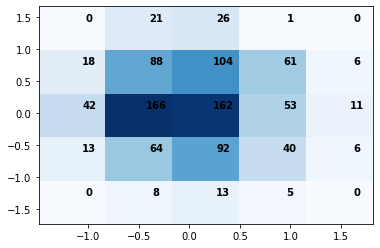
\includegraphics[scale=0.65]{hist.png}
\end{figure}\\
так как $n = 1000$, то $k = \frac{1000^{\frac{1}{3}}}{2} = \frac{10}{2} = 5$\\
Проверим методом $\chi^2$ гипотезу независимости компонент двумерного случайного вектора\\
(для этого используем scipy.stats.chi2\_controgency), получим:
\begin{verbatim}
    p-value: 0.0013793302370199627
\end{verbatim}
То есть p\_value $< 0.05$
\vskip 0.1in \noindent
Проверим гипотезы\\
Спирмен (используя scipy.stats.spearmanr): 
\begin{verbatim}
    coef = -0.03174930822554785
    p-value = 0.3158616269449295
\end{verbatim}
Пирсон (используя scipy.stats.pearsonr): 
\begin{verbatim}
    coef = -0.03618320814722287
    p-value = 0.2529735138640905
\end{verbatim}
\vskip 0.3in



\subsection*{Задача 2}
Проверми КС-методом гипотезу о совпадении законов распределения компонент вектора\\
(используя scipy.stats.ks\_2samp), получим:
\begin{verbatim}
    Ks\_2sampResult(statistic=0.06, pvalue=0.05462666510701526)
\end{verbatim}
Так как pvalue > 0.05, то законы не совпадают, но, что видно из значения, довольно близки
\vskip 0.2in \noindent
Распределение модулей похоже на полунормальное распределение (так как является модулем нормального)
\vskip 0.4in



\subsection*{Задача 3d}
Произведение плотностей точек $x_1, \ldots, x_n$ это $\frac{1}{\Gamma^n(r)} \cdot (x_1 \cdot \ldots \cdot x_n)^{r-1} \cdot e^{b(x_1 + \ldots + x_n)} \cdot b^{rn}$. Производная по b это $(nr - (x_1 + \ldots + x_n)b)e^{-(x_1 + \ldots + x_n)b} \cdot b^{nr-1}$, ее нули расположены в $0$ и $\frac{rn}{x_1 + \ldots + x_n}$, тогда максимум функции правдоподобия достигается при $b = \frac{rn}{x_1 + \ldots + x_n}$
\vskip 0.4in



\subsection*{Задача 4a}
Смесь плотностей имеет вид $\omega(\alpha) = \int\limits_{\mathbb{R}} v(\alpha, \theta) u(\theta) d \theta$ и $A| \Theta \sim \mathcal{U}(0; \Theta),\ \Theta \sim \mathcal{U}(0; 1)$, тогда
\begin{gather*}
    \int\limits_{\mathbb{R}} v_{A|\Theta}(\alpha, \theta) u_{\Theta}(\theta) d \theta
    = \int\limits_{0}^{\alpha} 0 d \theta + \int\limits_{\alpha}^{1} \frac{1}{\theta} d \theta
    = -\ln(\alpha)
\end{gather*}
То есть $w(x) = -\ln(x)$



\end{document}